% \iffalse
\let\negmedspace\undefined
\let\negthickspace\undefined
\documentclass[journal,12pt,twocolumn]{IEEEtran}
\usepackage{cite}
\usepackage{amsmath,amssymb,amsfonts,amsthm}
\usepackage{algorithmic}
\usepackage{graphicx}
\usepackage{textcomp}
\usepackage{xcolor}
\usepackage{txfonts}
\usepackage{listings}
\usepackage{enumitem}
\usepackage{mathtools}
\usepackage{gensymb}
\usepackage{comment}
\usepackage{tikz}
\usepackage[breaklinks=true]{hyperref}
\usepackage{tkz-euclide} 
\usepackage{listings}
\usepackage{gvv}
\def\inputGnumericTable{}
\usepackage[latin1]{inputenc}                              
\usepackage{color}                                            
\usepackage{array}                                            
\usepackage{longtable}                                       
\usepackage{calc}                                             
\usepackage{multirow}                                         
\usepackage{hhline}                                           
\usepackage{ifthen}                                           
\usepackage{lscape}

\newtheorem{theorem}{Theorem}[section]
\newtheorem{problem}{Problem}
\newtheorem{proposition}{Proposition}[section]
\newtheorem{lemma}{Lemma}[section]
\newtheorem{corollary}[theorem]{Corollary}
\newtheorem{example}{Example}[section]
\newtheorem{definition}[problem]{Definition}
\newcommand{\BEQA}{\begin{eqnarray}}
\newcommand{\EEQA}{\end{eqnarray}}
\newcommand{\define}{\stackrel{\triangle}{=}}
\theoremstyle{remark}
\newtheorem{rem}{Remark}
\begin{document}

\bibliographystyle{IEEEtran}
\vspace{3cm}

\title{ANALOG 11.14 Q-25}
\author{EE23BTECH11207 -KAILASH.C$^{*}$% <-this % stops a space
}
\maketitle
\newpage
\bigskip

\renewcommand{\thefigure}{\theenumi}
\renewcommand{\thetable}{\theenumi}
\textbf{QUESTION:}\\
A mass attached to a spring is free to oscillate, with angular velocity $\omega$, in a horizontal
plane without friction or damping. It is pulled to a distance $x_0$
 and pushed towards
the centre with a velocity $v_0$
 at time t = 0. Determine the amplitude of the resulting
oscillations in terms of the parameters $\omega{}$, $x_0$,
 and $v_0$
. [Hint : Start with the equation
$x = a \cos(\omega{t}+\theta{})$ and note that the initial velocity is negative.]\\

\textbf{SOLUTION:}\\
\begin{enumerate}
\item \textbf{Input Parameters:}
\begin{table}[h]
\begin{tabular}{|l|l|}
\hline
\textbf{Symbols} & \textbf{Definition}\\ \hline
$x$ & Displacement \\ \hline
$t$ & Time \\ \hline
$v$ & Velocity\\ \hline
$\omega$ & Angular velocity   \\ \hline
$\theta$ & Phase constant\\ \hline
$m$ & Mass\\ \hline
$a$ & Acceleration\\ \hline
$k$ & Force constant\\ \hline
\end{tabular}
\end{table}\\
\item \textbf{Free Body Diagram of Spring system:}
    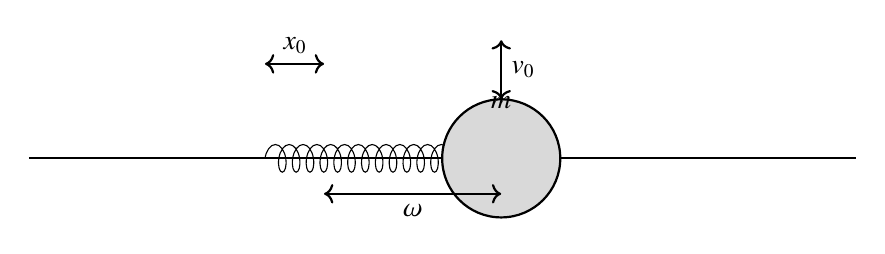
\begin{tikzpicture}[scale=1.5]
  % Ground
  \draw[thick] (-2,0) -- (5,0);

  % Spring
  \draw[decorate,decoration={coil,segment length=5pt,amplitude=5pt}] (0,0) -- (2,0);

  % Mass
  \draw[thick,fill=gray!30] (2,0) circle (0.5) node[above=0.5cm] {$m$};

  % Dashed line for equilibrium position
  \draw[dashed] (0,0) -- (0.5,0);

  % Arrows and labels
  \draw[<->,thick] (0,0.8) -- node[above] {$x_0$} (0.5,0.8);
  \draw[<->,thick] (2,1) -- node[right] {$v_0$} (2,0.5);
  \draw[<->,thick] (0.5,-0.3) -- node[below] {$\omega$} (2,-0.3);
\end{tikzpicture}\\
\item{}
From Newtons second law of Motion,
\begin{align}
    F&=ma 
\end{align}
We also know that From Hooke's Law, 
\begin{align}
F&=-kx
\end{align}
By equation-(1) and (2):
\begin{align}
    ma&=-kx\\
    m(\frac{dx^2}{dt^2})&=-kx\\
    \frac{dx^2}{dt^2}&=\frac{-kx}{m}
\end{align}
We know that $\omega=\sqrt{\frac{k}{m}}$
\begin{align}
    \frac{dx^2}{dt^2}&=-\omega^2x\\
    \frac{dx^2}{dt^2}+\omega^2x&=0
    \end{align}
\item{}
It is given that $\frac{dx}{dt}=-v_0$ at t=0s\\
By using the laplace trasnformation formula:$L(f"(t))=s^2L(f(t))-sf(0)-f'(0)$ provided that $s>0$ and  
By taking Laplace transformation in eq-(7),
\begin{align}    
(s^2 + \omega^2)X(s) - sx_0 - v_0&=0\\
X(s) &= \frac{sx_0 + x'_0}{s^2 + \omega^2}
\end{align}
Let us assume that the shm equation for displacement is:
\begin{align}
    x&=A(\cos{\omega t}+\theta)
\end{align}
Substituting eq-(10) in eq-(9):
\begin{align}
    X(s)&=\frac{s(A{\cos{\theta}})+x'(0)}{s^2 + \omega^2}\\
    v_0&=\frac{dx_0}{dt}\\
    v_0&=-A\omega{}\sin(\theta{})
\end{align}
Using eq-(13) in eq-(11):
\begin{align}
     X(s)&=\frac{s(A{\cos{\theta}})+A\omega{}\sin(\theta{})}{s^2 + \omega^2}\\
     X(s)&= \frac{A(s\cos(\theta) + \omega \sin(\theta))}{(s + i\omega)(s - i\omega)} \\
     X(s)&= \frac{A}{2i\omega} \left(\frac{1}{s - i\omega} - \frac{1}{s + i\omega}\right)
\end{align}
Using the inverse laplace transformation Formulas:\\
IL($\frac{1}{s-i\omega}$)=$e^i^\omega^t$ and 
IL($\frac{1}{s+i\omega}$)=$e^{-i\omega{t}}$,\\
We apply Inverse Laplace Transformation in eq-(16):
\begin{align}
X(s) &= \frac{A}{i\omega} (e^{i\omega t} - e^{-i\omega t}) \\
x(t)&= \frac{A}{i\omega} \sin(\omega t)\\
x(t)&=\frac{-iA\sin{\omega{t}}}{\omega}
\end{align}
Since $\sin(\omega{t})=\sin(\omega{t}+\pi)$ we can write eq-(19) as:
\begin{align}
     x(t)= A \cos(\omega t + \theta)
\end{align}
Hence it is the correct displacement equation
\item{}
Let at time t=0s, x=$x_0$\\
Substituting t=0s in equation (20):
\begin{align}
x&=A\cos(\omega{(0)}+\theta{})\\
x_0&=A\cos(\theta{})\\
v_0&=\frac{dx_0}{dt}\\
v_0&=-A\omega{}\sin(\omega{(0)}+\theta{})\\
v_0&=-A\omega{}\sin(\theta{})\\
-A\sin(\theta{})&=\frac{v_0}{\omega{}}
\end{align}
Squaring and Adding eq-(22) and eq-(25):\\
\begin{align}
(A\cos(\theta{}))^2+(A\sin(\theta{})^2)
&=(x_0)^2+\left(\frac{v_0}{\omega{}}\right)^2\\
A^2(\cos^2(\theta{})+\sin^2(\theta{}))
&=(x_0)^2+\left(\frac{v_o}{\omega{}}\right)^2\end{align}
\begin{align}
A^2=(x_0)^2+(\frac{v_o}{\omega{}})^2
\end{align}
\end{enumerate}\\
\textbf{Answer:}\\
Amplitude of the resulting oscillation is:$\sqrt{(x_0)^2+(\frac{v_0}{\omega{}})^2}$
\end{document}

